\documentclass{standalone}
\usepackage{graphicx}	
\usepackage{amssymb, amsmath}
\usepackage{color}

\usepackage{tikz}
\usetikzlibrary{intersections, backgrounds, math, decorations.pathreplacing}
\usepackage{pgfmath}

\definecolor{light}{RGB}{220, 188, 188}
\definecolor{mid}{RGB}{185, 124, 124}
\definecolor{dark}{RGB}{143, 39, 39}
\definecolor{highlight}{RGB}{180, 31, 180}
\definecolor{light_teal}{RGB}{107, 142, 142}
\definecolor{mid_teal}{RGB}{72, 117, 117}
\definecolor{dark_teal}{RGB}{29, 79, 79}
\definecolor{gray10}{gray}{0.1}
\definecolor{gray20}{gray}{0.2}
\definecolor{gray30}{gray}{0.3}
\definecolor{gray40}{gray}{0.4}
\definecolor{gray50}{gray}{0.5}
\definecolor{gray60}{gray}{0.6}
\definecolor{gray70}{gray}{0.7}
\definecolor{gray80}{gray}{0.8}
\definecolor{gray90}{gray}{0.9}
\definecolor{gray95}{gray}{0.95}

\begin{document}

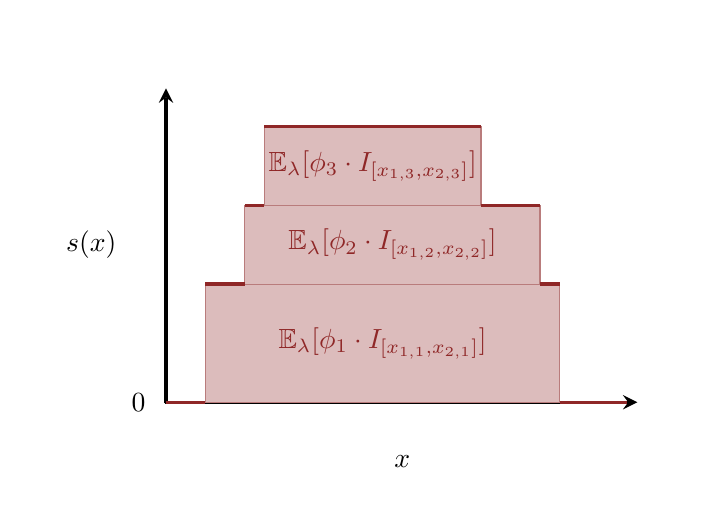
\begin{tikzpicture}[scale=1.0]

  \draw[white] (-4.75, -3.25) rectangle (3.5, 2.75);
  
  \draw [->, >=stealth, line width=1.25] (-3.00, -2.015) -- +(0, 4);
  \draw [->, >=stealth, line width=1.25] (-3.015, -2.00) -- +(6, 0);
  
  \filldraw[fill=light, draw=mid] (-2.5, -2) rectangle (2, -0.5);
  \node[dark] at (-0.25, -1.25) { $\mathbb{E}_{\lambda} [ \phi_{1} \cdot I_{[x_{1, 1}, x_{2, 1}]} ]$ }; 
  
  \filldraw[fill=light, draw=mid] (-2, -0.5) rectangle (1.75, 0.5);
  \node[dark] at (-0.125, 0) { $\mathbb{E}_{\lambda} [ \phi_{2} \cdot I_{[x_{1, 2}, x_{2, 2}]} ]$ }; 

  \filldraw[fill=light, draw=mid] (-1.75, 0.5) rectangle (1, 1.5);
  \node[dark] at (-0.375, 1) { $\mathbb{E}_{\lambda} [ \phi_{3} \cdot I_{[x_{1, 3}, x_{2, 3}]} ]$ }; 
  
  \draw[dark, line width = 1.25] (-3, -2) -- (-2.5, -2);
  \draw[dark, line width = 1.25] (-2.5, -0.5) -- (-2, -0.5);
  \draw[dark, line width = 1.25] (-2, 0.5) -- (-1.75, 0.5);
  \draw[dark, line width = 1.25] (-1.75, 1.5) -- (1, 1.5);
  \draw[dark, line width = 1.25] (1, 0.5) -- (1.75, 0.5);
  \draw[dark, line width = 1.25] (1.75, -0.5) -- (2, -0.5);
  \draw[dark, line width = 1.25] (2, -2) -- (2.85, -2);
  
  \node at (-3.35, -2) { $0$ };
  \node at (-3.95, 0) { $s(x)$ };
  
  
  \node at (0, -2.75) { $x$ };

  
\end{tikzpicture}

\end{document}  